\begin{tikzpicture} [scale= .35]
	\draw node at (-4,0){ };
	\draw node at (4,0){ };
	\draw[fill] (-0.4,0) circle  [radius=3pt];

	\draw node at (-0.4,1){$n=0$} ;
	\draw node at (0,-2.4){} ;
\end{tikzpicture}
\begin{tikzpicture} [scale= .35]
	\draw[fill] (-4,0) circle  [radius=3pt];
	\draw[fill] (4,0) circle  [radius=3pt];

	\draw [->] (-4,0) [shorten >=0.2cm, shorten <=0.2cm,->] to (4,0) ;

	\draw node at (0,1){$n=1$} ;
	\draw node at (-6,-2.4){} ;
\end{tikzpicture}

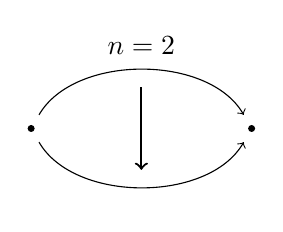
\begin{tikzpicture} [scale= .35]
	\draw[fill] (-4,0) circle  [radius=3pt];
	\draw[fill] (4,0) circle  [radius=3pt];

	\draw [->] (-4,0) [shorten >=0.2cm, shorten <=0.2cm,->, out=60,in=120] to (4,0) ;
	\draw [->] (-4,0) [shorten >=0.2cm, shorten <=0.2cm,->, out=-60,in=-120] to (4,0) ;

	\draw [->] (0,1.5) [thick] to (0,-1.5) ;

	\draw node at (0,3){$n=2$} ;
\end{tikzpicture}
\hspace*{25pt}
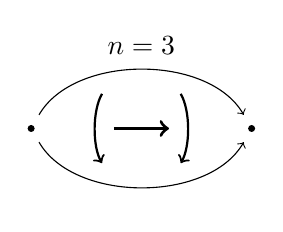
\begin{tikzpicture} [scale= .35]
	\draw[fill] (-4,0) circle  [radius=3pt];
	\draw[fill] (4,0) circle  [radius=3pt];

	\draw [->] (-4,0) [shorten >=0.2cm, shorten <=0.2cm,->, out=60,in=120] to (4,0) ;
	\draw [->] (-4,0) [shorten >=0.2cm, shorten <=0.2cm,->, out=-60,in=-120] to (4,0) ;

	\draw [->] (-1,2) [thick,shorten >=0.3cm, shorten <=0.3cm,->, out=-120,in=120] to (-1,-2) ;
	\draw [->] (1,2) [thick,shorten >=0.3cm, shorten <=0.3cm,->, out=-60,in=60] to (1,-2) ;

	\draw [->] (-1,0) [very thick] to (1,0) ;

	\draw node at (0,3){$n=3$} ;
\end{tikzpicture}